\documentclass[12pt]{article} 
\usepackage{listings}

\usepackage[pdftex]{graphicx}
\usepackage{setspace}
\newcommand{\HRule}{\rule{\linewidth}{0.5mm}}
\onehalfspacing
\pdfpagewidth 9in
\setlength{\topmargin}{1in}
\setlength{\headheight}{0in}
\setlength{\headsep}{0in}
\setlength{\textheight}{7.7in}
\setlength{\textwidth}{6.5in}
\setlength{\oddsidemargin}{0.5in}
\setlength{\evensidemargin}{0in}

\usepackage{color}
\usepackage{xcolor}
\usepackage{listings}
\usepackage{graphicx}
\usepackage{moreverb}
\usepackage{caption}
\usepackage{makeidx}
\usepackage[toc,style=treenoname,order=word,acronym]{glossaries}
\makeindex


\usepackage{glossaries}
\makeglossaries



\DeclareCaptionFont{white}{\color{white}}
\DeclareCaptionFormat{listing}{\colorbox{gray}{\parbox{\textwidth}{#1#2#3}}}
\captionsetup[lstlisting]{format=listing,labelfont=white,textfont=white}

\newglossaryentry{cocoatouch}{name=cocoa touch,
description= An API for developing user interfaces for iOS devices}
\newglossaryentry{udp}{name=UDP,
description= user datagram protocol}
\newglossaryentry{tcp}{name=TCP,
description= Transmission control protocol}
\newglossaryentry{soap}{name=SOAP,
description=  Simple object access protocol}
\newglossaryentry{rest}{name=REST,
description= Representational state transfer}
\newglossaryentry{http}{name=HTTP,
description= Hyper Text Transfer Protocol}
\newglossaryentry{mapkit}{name=MapKit,
description= Framework for developing map applications for iOS devices}
\newglossaryentry{socket}{name=socket,
description= Endpoint for communicaition in networks}
\newglossaryentry{synchronous}{name=Synchronous Request ,
description= Request to remote server where further code cannot be executed until the request has finished }
\newglossaryentry{ocunit}{name=OCUnit ,
description= Request to remote server where further code cannot be executed until the request has finished }
\newglossaryentry{asynchronous}{name=Asynchronous Request,
description=Request which is non blocking where further code can be executed without waiting.}
\newglossaryentry{uimage}{name=UIImagePickerController ,
description= {class manages customisable, system-supplied user interfaces for taking pictures and movies on supported devices, and for choosing saved images and movies for use in your app. An image picker controller manages user interactions and delivers the results of those interactions to a delegate object.} }
\newglossaryentry{sdk}{name=SDK ,
description={Software development kit. When spoken about in this document referring the the iPhone OS SDK. This is a software development kit which provides tools to develop iPhone applications. The development kit is available to third party developers.} }

\newglossaryentry{ibaction}{name=IBAction ,
description={ Identifier used to qualify an instance-variable declaration so that Interface Builder can synchronize the display and connection of outlets with Xcode. } }
\newglossaryentry{sqlite}{name=sqlite,
description= {a software library that implements a self-contained, serverless, zero-configuration,transactional SQL database engine. } }

\newglossaryentry{nsdefault}{name=NSUserDefaults,
description= {Provides access to the default settings in the device.} }

\newglossaryentry{mysql}{name=MySQL,
description= {Relational Database management system } }

\newglossaryentry{iphone}{name=iPhone ,
description= {A line of internet and multimedia enabled smartphones designed and marketed by Apple inc. } }

\newglossaryentry{cfnetwork}{name=CFNetwork ,
description= {A framework in the Core Services framework that provides a library of abstractions for network protocols.. } }

\newglossaryentry{coreloc}{name=Core Location,
description= {The Core Location framework lets you determine the current location or heading associated with a device. } }

\newglossaryentry{3gs}{name=3GS ,
description= {Third generation of the iPhone } }

\newglossaryentry{appstore}{name=App Store ,
description= {An application used on iPhone devices to download native and third party applications } }


\newglossaryentry{asihttp}{name=ASIHTTPRequest ,
description= {an easy to use wrapper around the CFNetwork API that makes some of the more tedious aspects of communicating with web servers easier. } }


\newglossaryentry{smartphone}{name=Smartphone ,
description= {A telephone that provides additional information accessing features. Any mobile telephone that combines voice services with e-mail, fax, pager or Internet access is called a smart phone. } }
\newglossaryentry{ios}{name=iOS,
description= {Stands for iPhone Operating System is a mobile operating system for use with Apple mobile devices.  } }
\newglossaryentry{geocaching}{name=Geocaching ,
description= {A pastime in which objects are hidden at secret locations for participants to find using GPS positions posted on the Internet. }, plural=Linuces }
\newglossaryentry{app}{name=app ,
description= {Short for application, refers to applications used by the iPhone or other smartphone devices. } }
\newglossaryentry{api}{name=API ,
description= {Set of rules or specifications which a software program can follow. } }
\newglossaryentry{objectc}{name=Objective C,
description= {Object oriented programming language } }
\newglossaryentry{ui}{name=UI ,
description= { User interface } }
\newglossaryentry{gps}{name=GPS ,
description= {Global positioning system } }
\newglossaryentry{googlemaps}{name=Google Maps ,
description= {A web mapping service provided by Google } }

\newglossaryentry{xcode}{name=XCode,
description= {Development environment for Mac OS applications } }

\newglossaryentry{php}{name=PHP,
description= {Server side scripting language which is HTML embedded. } }

\newglossaryentry{ftp}{name=FTP,
description= {File Transfer Protocol. Network protocol used to transfer files } }
\newglossaryentry{macos}{name=Mac Os X,
description= {Unix based operating system developed by Apple} }


\begin{document}

\begin{titlepage}

\begin{center}

% Upper part of the page
   
\textsc{\LARGE University of Limerick}\\[1.5cm]

\textsc{\Large Final year project}\\[0.5cm]

\textsc{\Large Interim Report}\\[0.5cm]

% Title
\HRule \\[0.4cm]
{ \huge \bfseries GeoTrash}\\[0.4cm]
{ \small \bfseries Litter Tracking Smartphone Application}\\[0.4cm]

\HRule \\[1.5cm]

% Author and supervisor
\begin{minipage}{0.4\textwidth}
\begin{flushleft} \large
\emph{Author:}\\
\textsc{Patrick Russell - 0734004}
\end{flushleft}
\end{minipage}
\begin{minipage}{0.4\textwidth}
\begin{flushright} \large
\emph{Supervisor:} \\
Mr.~Michael \textsc{Coughlan}
\end{flushright}
\end{minipage}

\vfill

% Bottom of the page
{\large \today}

\end{center}

\end{titlepage}
%Acknowledgements

\newpage

\label{sec:Acknowledgements}
\section{Acknowledgements}
\paragraph{}
I am thankful to my supervisor Micheal Coughlan for helping to shape the project by providing ideas on the project structure. I would like to offer my thanks to Gabriella Avram for providing the original project specification, although the project has been changed greatly from this original specification many of the core ideas have been held. 
I would like to thank my friends for helping me with ideas, advice and support throughout implementation of the project. 


\newpage

% Table of contents

\tableofcontents
\newpage

% Summary Section


\section{Introduction}
\paragraph{}


\subsection{General Introduction}

A smartphone is a telephone that provides additional information accessing features. Any mobile telephone that combines voice services with e-mail, fax, pager or Internet access is called a smart phone. The majority of smartphones have the ability to install third party applications, the core focus of this project is an application for one of these smartphone devices. The device chosen was an \gls{iphone} \gls{3gs} with \gls{ios} 4.2.

\paragraph{}


This project is a \gls{geocaching} iPhone application targeted at trying to reduce litter. The application works by the user taking a picture of a piece of litter and uploading it to a remote server.
This photo can then be uploaded to a remote server along with the location of the device at the time of taking the photo. This data can then be used by other users to identify litter blackspots and help councils perform cleanups in the area.

\paragraph{}


The project is divided into three areas these are the iPhone application, the web services implementation and the website. The application was developed for the \gls{ios} platform for \gls{iphone} devices in particular. The application will allow users to take pictures of litter and upload them to a remote database. The geographical location will be stored with this picture on the server and can be displayed on a map by other users. Users can select points on this map and view the photo and details about it. A website will provide a web based  representation of the data captured by the application. A map similar to the one on the application itself will be represented with points representing litter location and the image.

\paragraph{}


The platform chosen for development was the iPhone running \gls{ios} 4.2. The development environment chosen was \gls{xcode} as it is required for \gls{ios} development. The language chosen was \gls{objectc} which is also a requirement for iOS. The UI design was done using interface builder which is a part of Xcode and is designed for designing interfaces for \gls{ios} devices. The project also needed to have a remote database to store photos and \gls{gps} locations. For this a \gls{mysql} web server is required along with web services to allow the device to input and retrieve data from this database. Some \gls{php} code was also utilised to handle the web services. The \gls{googlemaps} \gls{api} is used on the Website to represent the data in the database on a map for users on a computer to view. The Website will also need to have the function to view and manage photos and account information.

\paragraph{}

This project is an application for a \gls{smartphone} targeted at reducing litter and promoting cleanliness. This application will work by a user locating a piece of litter taking a picture of it. The location of the device when the picture is taken will correspond to the location of this particular piece of litter. This data must be stored in a remote database and can be viewed by other users.

\paragraph{}

It is a requirement that the application be written in \gls{objectc} as this is the language which is used to develop for \gls{ios}. \gls{ios} is a branch of the C programming language so it bears some resemblance to languages such as C or C++ however it differs in quite a lot of areas. This is a small factor as some time had to be spent to learn this language before beginning. There is also a development environment for Mac OS and \gls{ios} applications and this is \gls{xcode}. The environment also incorporates a \gls{ui} editor and a simulator to test applications.

\paragraph{}


A database will need to be implemented to store user/device identies, photos with their geographical location and possibly some other information which would be necessary. I propose to do this by creating an SQL database which the device can connect to to pull and push data as necessary using web services.

\paragraph{}

The data collected using the application can also be represented on a Website for the users to as with the application view photos and litter spots. Using the location details it will be possible to represent the areas which have high concentration of litter using this Website to highlight key areas so that authorities can take necessary action to reduce the litter.

\newpage




%Motivation Factors


\subsection{Motivation Factors}

When choosing my area of focus for my FYP I wanted to focus on an area which interests me while also including the skills which I learned during my degree programme. My programming knowledge was quite good when starting the project however this project brought in a new language which I had not experience with. This is important for future programming work as technology changes quite quickly in the software world so it is important to be versatile.
I wanted also to learn about remote data, having data in the “cloud” is becoming popular in recent times so learning about how this can be done is important. 
Skills in web development are always useful to have so the website part of the project provides an insight here.


%Objectives Of Proposed Work

\subsection{Objectives of Proposed Work}

The objectives of the project are to implement an integrated system based on web an \gls{smartphone} application technologies. The project was outlined to have the functionality which was set out in the introduction section but also have a high quality \gls{ui} and very stable code. Before deciding on the areas of focus on the project I set out to examine similar applications and possible implementation methods. A summary of these findings are outlined in chapter 2. Chapter 3 will outline the design of the system while chapter 4 will outline how this was implemented chapter 5 will present the results of testing the software. Finally chapter 6 will conclude the findings of the project and make recommendations.   


\newpage


%Research

\section{Research}

%Geo Caching

\subsection{Geo Caching}

\gls{geocaching} as described by techtarget.com: "\gls{geocaching}, also referred to as \gls{gps} stash hunting, is a recreational activity in which someone "buries" something for others to try to find using a Global Positioning System (\gls{gps} ) receiver."
The \gls{iphone} application store or \gls{appstore} contains hundreds of thousands of applications so it was not hard to locate one which provides similar functionality to this project.
There are many \gls{geocaching}  applications available currently available for smartphones.
One of these applications is simply called \gls{geocaching} . This is a global treasure hunting game where participants hide and seek physical containers called geocashes and they share their adventures online.
After observing this application some inspiration was taken from it. First of all the \gls{ui}  was quite good and the layout is something which will be taken into account when it comes to designing the \gls{ui} . The functionality of this application also provided an insight. \gls{geocaching}  allows you to place an object on the map in the application and the position of this object is uploaded to their remote server. This is very similar to what needs to be done for this project. The project also has a map where you can view nearby \glspl{geocaching} this functionality would be a useful addition to the project.



%Platforms http://whatis.techtarget.com/definition/0,,sid9_gci1131231,00.html

\subsection{iPhone Development}
There are many development tutorials on the Internet which provide sample code for projects which contain some of the functionality which is required for this project. One of these sample applications is one which takes control of the camera on the phone. The application shows a view which is the live feed from the camera. This application utilises the \gls{uimage} class from the \gls{iphone} \gls{sdk} library. With this class you can decide how you want the camera view to appear and choose whether you want controls for taking photos by specifying it in the code. The \gls{uimage} class is defiantly going to be an important part of the project.



\paragraph{}
\label{par:First Paragraph}

Another important factor in developing the application is obtaining a geographical location. Obtaining the location is done using the \gls{coreloc} Framework. This framework provides access to all of the iPhones location systems. These include integrated \gls{gps}, Wifi-based location positioning and tower triangulation.
A sample application was located which will simply display the latitude and longitude on the screen. When obtaining a location there are a number of query parameters which need to be considered one which will need to be taken into consideration is the desired accuracy parameter. The reason accuracy will need to be specified is to conserver battery and to avoid unnecessary updates by having only a level of accuracy which is required.

\paragraph{}
\label{par:First Paragraph}

Another important consideration for the application is the persistence of data, it needs to be decided whether a certain amount of state be saved when the application is closed. Data such as user log in data will need to be saved. This data is usually stored in a location which is designated for saving user data. This memory is referred to by calling the \gls{nsdefault} class where you can store data of different data types.

\subsection{User Interface}

The user interface is an important design element in the project. As observed from using \gls{xcode} to develop some sample applications a tool is available for user interface design. This is known as the interface builder which is a part of the Xcode development environment. With this application you can create and edit views. A view is in simplest terms is what is displayed on a screen at a given moment during the execution of an application, an application can have one or multiple views. The \gls{iphone} utilises the \gls{cocoatouch} \gls{api}. \gls{ios} technologies can be seen as a set of layers, \gls{cocoatouch} is seen as the highest level and the Core OS and \gls{macos} kernel at the bottom. The advantage of this layer is that it makes the implementation of applications easier because the developer is not concerned with things such as how to recognise if a button was pressed. The interface builder contains a library of elements which will be discussed in the design section.

\subsection{Web Services}

There are various ways in which the data can be sent and received from the remote server. To handle the passing of data between phone and database a web service such as \gls{soap} or \gls{rest} would need to be implemented. The iPhone \gls{sdk} incorporates the \gls{cfnetwork} framework this framework makes it possible to communicate across network sockets using either \gls{udp} or \gls{tcp}.  \gls{tcp} sockets will be used for this project as it is important data is not lost in transmission. The \gls{cfnetwork} framework also provides support for \gls{http} and \gls{ftp} which makes the utilisation of web services possible.

\paragraph{}

Although the \gls{cfnetwork} \gls{cfnetwork} provides all the required functionality \gls{asihttp} is a wrapper which is used around the \gls{cfnetwork} \gls{api}. This wrapper can be used to make it easier to do the more tedious tasks associated with communication with the web server. There are some features of this wrapper which may be beneficial to the project.

\paragraph{}

Features of \gls{asihttp}:
\begin{itemize}
\item A straightforward interface to submitting data to and fetching data from webservers.
\item Download data to memory or directly to a file on disk.
\item Easy to access request and response \gls{http} headers.
\item Progress delegates to show information about download and upload progress.
\end{itemize}

\paragraph{}
Since it is a requirement that data be uploaded to a web server the above functionality would be quite beneficial in that it would take the tedious nature out of completing the task of uploading.
It will also be important to retrieve information such as success information for uploaded data and retrieving data from the server using a request. The easy access to request response \gls{http} headers will be beneficial here. Obtaining data from the remote server will not be an instant process as regards the users interaction. For that reason progress delegates can be used to show the user how long is left to wait before progression. 

\paragraph{}
With web services there also comes the issue of storing the data. The method decided upon is using a \gls{mysql} server. The reason for this is that it integrates well with web services but more importantly the database can be accessed by other media such as a Website which is an important factor for this project.



%Software and Language http://mobileorchard.com/hello-there-a-corelocation-tutorial/

\subsection{Data Persistence}

This section will disuss the persisesnce of data in the application with focus on the data which is retrieved from the remote database. When data is obtained from the remote database it is possible to just store it within variables in running code. This would be the easiest solution it seems however there are disadvantages to doing this such as updates would have to be done regularly as data may need to be moved from memory if the application was shut for example. When in an area with no data connection this solution would limit the application to areas within wifi coverage or cellular data connections. 

\paragraph{}


A solution to this problem would be the implementation of a local database which is essentially a copy of the remote one. Some research was done into how this data might be stored. The \gls{ios} provides support for sqlite databases. sqlite is a software library that implements a self-contained, serverless, zero-configuration,transactional SQL database engine. 

\paragraph{}

\gls{sqlite} is an embedded database library that implements a large subset of the SQL 92 standard. Its claim to fame is the combination of both the database engine and the interface (to said engine) within a single library, as well as the ability to store all the data in a single file. I terms of functionality \gls{sqlite} resides somewhere between \gls{mysql} and PostgreSQL. However, when it comes to performance, \gls{sqlite} is often 2-3 times faster (or even more). This is thanks to a highly tuned internal architecture, and the elimination of server-to-client and client-to-server communication. 

\paragraph{}

All this is combined into a package that is only slightly larger than the \gls{mysql} client library, an impressive feat considering you get an entire database system with it. Utilizing a highly efficient memory infrastructure, \gls{sqlite} maintains its small size in a tiny memory footprint, far smaller then that of any other database system. This makes \gls{sqlite} a very handy tool that can efficiently be applied to virtually any task requiring a database.


%Application map

\subsection{Application Map}

A map is also a requirement for the application as it is important for the user to be able to browse the map to search for litter.
Maps can be added to a view in the application similar to above using the \gls{mapkit} framework. A map can be added to a view which displays the current location to a specified range. The user can also pinch and drag to move the current position in vision on the map. There is also the issue of adding a marker to the map to display where there is an item of litter. The \gls{mapkit} framework also provides the function of adding what are called pins, they are simply markers on the map. It is also possible to put code behind one of these pins. This can be used when a user selects a pin a page can load showing the image of the piece of litter and some other basic information.
There are various test applications on developer.apple.com/iphone which incorporate \gls{mapkit}. The application consists of a basic map view which shows the current location. It will also place markers on the screen relative to previous visited locations.


\subsection{Website Map}

The most popular maps which are used on most websites use the google maps API. Code.google.com provides an explanation of all the different \gls{api} family items. 
Google maps API Family:
\begin{itemize} 
\item{} Maps JavaScript API
\item{} Maps API for Flash
\item{} Google Earth API
\item{} Static Maps API
\end{itemize}

\paragraph{}
\label{par:First Paragraph}

A choice must be made here as to which is the best option to implement with. The requirements of the chosen option are that an the map is interactive and is able to display markers showing litter spots. The option must also enable these points to be selected displaying an image of the litter.

\paragraph{}
The static maps \gls{api} can be eliminated here as this option is not interactive. 

\paragraph{}
The javascript option provides all the required functionality mentioned above. The option also includes the option to view the map in Satellite view which would be a useful feature for users of the site. 

\paragraph{}
The Google Earth \gls{api} allows you to embed three dimensional views of maps. Although it is possible to provide all the functionality with this the three dimensional element is possibly more than is required for this project. 


\paragraph{}
The Flash \gls{api} is very similar to the javascript version mentioned above in that it provides satellite and basic map functions. The only significant difference to note would be the accessibility of flash v javascript, not all devices support flash but a great deal more support javascript.

% Design
\section{Design}

\subsection{Application}
\subsubsection{User Interface}
\paragraph{}


The user interface for the application required careful consideration before development. Taking into account the examples of other similar applications a user interface design was created. The key requirement of the user interface for this application was to keep it simple. This means limited buttons and menu items. The reasoning for this is that the application serves a simple purpose and it is important not to distract the user from the core functionality of the application.

\paragraph{}

Figure 1 shows a snap shot of the user interface of the main view. The bar along the bottom is a toolbar. Buttons may be added to this toolbar which perform actions. A simple text view displays an introduction to the application. A bar was chosen as the preferred method of navigation throughout the application as it is simple yet effective.

\paragraph{}
The map view will simply display a map utilising the google maps \gls{api}. There are no significant design elements in this view only that it keeps the navigation bar as before. 

The photo view which utilises the \gls{uimage} class. This is the only view in the project which the toolbar doesnt follow on the bottom of the screen. The reason for this is so the user will complete taking of the photo before they continue. 

The next view will display the image which was taken and ask the user if they wish to upload it. Figure 2 shows an example of how this will appear on screen. 

\paragraph{}

An image view was included in the main section of the application. This view required what is known as a referencing outlet. A referencing outlet is where the view will look for a particular piece of information. Here the theImageView object was referenced for image data. The interface builder also allows editing of colours, shapes and sizes etc. of all \gls{ui} elements. These tools were used in the final design of the look an feel of the application.

\paragraph{}

The instructions button will load a screen displaying text based instructions on how to use the application. Again here the toolbar is maintained along the bottom of the screen. Figure 3 shows what this view should look like.

\begin{figure}[htb]
\begin{center}
\leavevmode
\includegraphics{MainView}
\end{center}
\caption{Main View}
\label{fig:main_view}
\end{figure}

\begin{figure}[htb]
\begin{center}
\leavevmode
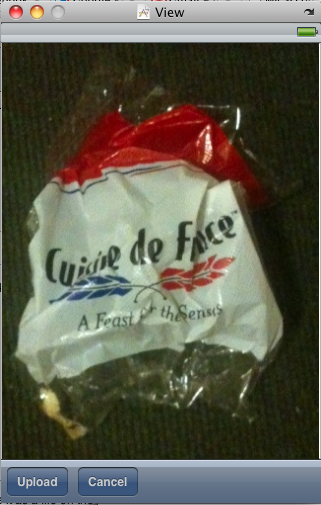
\includegraphics{upload}
\end{center}
\caption{Upload Image View}
\label{fig:upload}
\end{figure}

\begin{figure}[htb]
\begin{center}
\leavevmode
\includegraphics{instruct}
\end{center}
\caption{Instructions View}
\label{fig:instruct}
\end{figure}

\subsection{Maps}

The function of maps section of the application is to display a map which zooms to a level close to where the end user is, display a map which shows terrain and roads etc. The map must also display points which correspond to the location of the litter. Once one of these markers are selected an image which corresponds to the point must be displayed. 

\paragraph{}

The \gls{iphone} \gls{sdk} contains an \gls{api} for \gls{googlemaps} which is a native application on the phone. Displaying a map was done by loading a new view using the \gls{mapkit} framework.

\paragraph{}

There are a number of options which can be set upon loading a new map view. One of these is the showUserLocation method, when set to true this will display a dot corresponding to the users location. It is important to set the accuracy using the desiredAccuracy method. A highly accurate setting on this would cause unnecessary battery drainage due to the requirement that many sensors would have to be used. On the other hand an inaccurate setting would be misleading to the user as to their position so a compromise was made as to the decision. To the nearest ten meters was the setting which was decided upon. 

\paragraph{}

The next item for consideration was the points on the map which correspond to the litters location. The \gls{api} also contained a class for displaying these points and they are referred to as pins. An Annotation or pin may be added to the current map view by specifying a latitude and longitude. A number of annotations had to be loaded when the application started these points were loaded from the locally stored database then represented on the map once loaded. 
\subsection{Remote Database}


A decision had to be made as regards how long data stay present in the database. It was decided that the data remain in the database as it is not expected that there would be millions of records inserted. The application itself will be designed so that the application is not overloaded with data by limiting the amount of records displayed. The database needs to contain data pertaining to the location of the litter, timestamp the URL of the uploaded photo and the identiy of the device. The Database will be outlined as follows:
GeoTrash
ID
Timestamp
Latitude
Longitude
PhotoURL
DeviceID

\subsection{Web Services}

Sudocode for inserting:
\begin{verbatim}

int timestamp = currentTimestamp
int latitude = POST(lat)
int longitude = POST(lon)
int deviceID = POST(devid)

connectToDatabase()
INSERT INTO GeoTrash Values (timestamp, latitude, longitude, deviceID)
CloseDatabase()
\end{verbatim}
\begin{verbatim}
Sudocode for selecting:

result = SELECT * FROM GeoTrash WHERE 1=1
echo result;
\end{verbatim}
Deleting:

\begin{verbatim}
id = POST(ID)
sql = DELETE FROM GeoTrash WHERE ID = id
echo success
\end{verbatim}

\subsection{Application Back-End}

This section will discuss the implementation of the coding of the application. Figure 4 shows a class diagram of the application.

\subsubsection{Description Of Structure}

Image Picker:
The purpose of this class is to manage the initiation of a new photo view and carry out the photo taking operations. 

\paragraph{}
Annotation:
This will handle the points on the map referring to pieces of trash and the images connected with them.

\paragraph{}
Cacher:
This will handle updating of the local database.

\paragraph{}
GeoTrashViewController:
This will handle the UI elements of most of the application.

\paragraph{}
ImagePicker:
This will manage the taking of photos.

\paragraph{}
TrashPiece:
This will be an object which contains info for each trash piece which is currently in memory. Holding things like latitude, longitude etc.

\paragraph{}

The pink interfaces above show interfaces which are provided by the \gls{api} which are required for functionality by classes mentioned. 

\begin{figure}[htb]
\begin{center}
\leavevmode
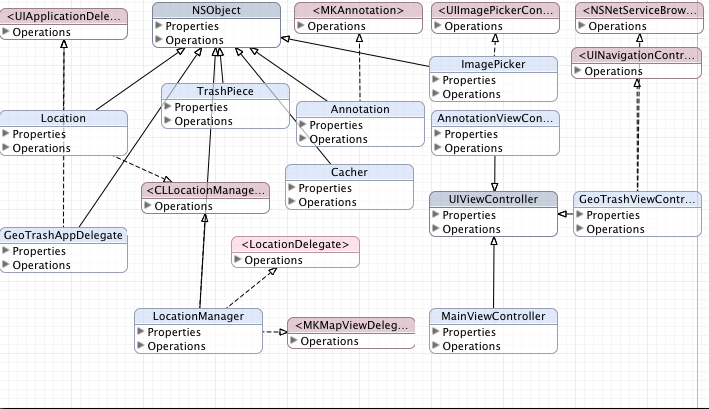
\includegraphics[scale =0.8 ,angle=90]{class}
\end{center}
\caption{Design Class Diagram}
\label{fig:class}
\end{figure}


\subsection{Web Services}
For the data to move between the web server and the application and the website web services had to be implemented. 

\section{Application}
\subsection{User Interface}

The design of the \gls{api} has been mentioned in a previous section this section will discuss the inner workings of the user interface and the issues which occurred during development.
\paragraph{}

Interface builder objects such as buttons have a predefined list of events which can occur on the object. These events can be linked up with classes in the code to be invoked by a chosen event. For button items the most commonly used event is “touch up inside” which causes an event when a button is pressed. The event can be linked up to classes with the \gls{ibaction} identifier in the project. 

\paragraph{}

Once the application is launched the first thing which happens is the GeoTrashViewController interface file is loaded to the screen. If the a photo option is selected the photo view is presented. Here is the code which causes this to happen:
\begin{verbatim}
-(IBAction) getPhoto:(id) sender{
	// load the image picker view
	UIImagePickerController * picker = [[UIImagePickerController alloc] init];
	picker.delegate = self;
	
	if((UIButton *) sender == sentPhoto) {
		picker.sourceType = UIImagePickerControllerSourceTypeSavedPhotosAlbum;
	} else {
		picker.sourceType = UIImagePickerControllerSourceTypeCamera;
	}
	//make visable
	[self presentModalViewController:picker animated:YES];
}
\end{verbatim}

\paragraph{}
The significance of IBAction here is that this piece of code is called when a specific event occurs in the interface. The first line is the allocation of memory and initialisation of the data for the picker object.
The options are set for the source type for camera. The view is then set to appear above the main view by setting animated to YES.
When this view is no longer needed or the user selects another menu option removeMapFromSuperview is called on the view object, this removes it from vision. Since it is the same implementation for adding and removing other views this document will not continue to explain how the other views were implemented.
theImageView refers to the image view object created in the interface builder. This view is invisible when there is no image connected with the view but after the user takes a photo this image is set in this line of code:
self.theImageView.image = [info objectForKey:@"UIImagePickerControllerOriginalImage"];
The UIImagePickerControllerOriginalImage key refers to the image which was taken using the image picker.

\subsection{Uploading Images}

This section will discuss uploading the image which was obtained from the image picker. imageUploader is the operation which handles this. 

\subsection{Building Local Database}

The local database contains the same rows as the remote database however when the application is started it contains no records. Once the application loads the following method is called:

\begin{verbatim}
- (void)populateLocationList:(id)sender
{
	cacher = [[Cacher alloc]init];
	id number;
	
	//[number locationsArray];	
	
	number = self.cacher;
    [number buildDatabaseFromRemoteData];
	
}
\end{verbatim}


This method creates a new cacher object and calls buildDatabaseFromRemoteData on the object. 
\begin{verbatim}
-(void)buildDatabaseFromRemoteData{
	
		
		// Starts the asynchronous request which calls for all the rubbish items from the remote server.
	
		locCache = [[NSMutableArray alloc] init];
		
	    NSArray *documentPaths = NSSearchPathForDirectoriesInDomains(NSDocumentDirectory, NSUserDomainMask, YES);
	    NSString *documentsDir = [documentPaths objectAtIndex:0];
	    databasePath = [documentsDir stringByAppendingPathComponent:databaseName];
	
		NSURL *url = [NSURL URLWithString:@"http://www.skynet.ie/~paruss/iPhone/getLocations.php"];
		ASIHTTPRequest *request = [ASIHTTPRequest requestWithURL:url];
		[request setDelegate:self];
		[request setDidFinishSelector:@selector(requestFinished:)];
		[request startAsynchronous];
		
		//check and create the database 
	
		[self checkAndCreateDatabase];
		
	}
\end{verbatim}

The code above starts an asynchronous request for the data in the remote database. The URL points to a PHP file which obtains data from the SQL server. The significance of it being an asynchrous request is so that the user does not have to wait while this is taking place. Once the request has finished requestFinished is called. This method will firstly check if the local database exists, if it does it will delete everything from it as this data may be old.
\begin{verbatim}
NSString *responseString = [request responseString];
		NSLog(@"Response: %@", responseString);
		NSArray *chunks = [responseString componentsSeparatedByString: @" "];
\end{verbatim}

The response from the request is loaded into a string. The data must then be split up by the spaces to separate the string into chunks containing individual records to be re-assembled to insert into the local database. The following is a snippet which performs the operation of iterating through the list of items and inserting them into the local database:
\begin{verbatim}
int count = [chunks count];
		//iterate through each item 
		int i = 0;
		
		while (count >= 3)
		{
			
			const char *sqlStatement = "insert into cache(id, timestamp, latitude, longitude) VALUES (?, ?, ?, ?)";
			
			if(sqlite3_prepare_v2(database, sqlStatement, -1, &addStmt, NULL) != SQLITE_OK)
				NSAssert1(0, @"Error while creating add statement. '%s'", sqlite3_errmsg(database));
			
			
			
	        int ID = [[chunks objectAtIndex:i] intValue];
			int ts = [[chunks objectAtIndex:i + 1] intValue];
			double lat = [[chunks objectAtIndex:i + 2] doubleValue];
			double lon = [[chunks objectAtIndex:i +  3] doubleValue];
			
			sqlite3_bind_int (addStmt, 1, ID);
			sqlite3_bind_int (addStmt, 2, ts);
			sqlite3_bind_double(addStmt, 3, lat);
			sqlite3_bind_double(addStmt, 4, lon);

\end{verbatim}

Once a photo has been taken the Upload method is called and is outlined here:

\begin{verbatim}
- (void)Update:(id)sender
	{
		NSString *latPost = self.lat;
		NSString *lonPost = self.lon;
		NSURL *url = [NSURL URLWithString:@"http://www.skynet.ie/~paruss/iPhone/Uploader.php"];
		ASIFormDataRequest *request = [ASIFormDataRequest requestWithURL:url];
		[request setPostValue:lonPost forKey:@"lon"];
		[request setPostValue:latPost forKey:@"lat"];
		[request start]; 
		NSError *error = [request error];
		if (!error) {
			
			NSString *response = [request responseString];
			NSLog(@"Output", response);
		}
	}


\end{verbatim}

From the code above we see that the URL is set for the request. The POST values are then set for the request. This code snippet uses the ASIHTTPRequest wrapper. The request is then started.
\paragraph{}
The map is loaded by loading a new map view similar to the photo views mentioned above. Once the map is loaded a dot will appear on screen displaying the current position of the device. The desiredAccuracy variable of the map view must be set to define how accurate the updating of the current position must be. The chosen value was to within ten metres. This is a value which is accurate enough for the user to identify nearby litter but not too accurate that it drains the battery in the device. Once the map is loaded all the values in the local database are loaded and the Annotations of the litter are placed on the screen. 

\subsection{Google Maps API}

The \gls{googlemaps} \gls{api} was chosen to represent litter data on a map for the website.  
The javascript API was chosen for embedding on the website. 
The data is retrieved from the server using web services which are implemented in \gls{php}. A request will be made to retrieve location coordinates. Once returned they are loaded into the javascript code to be displayed on the map. 

\paragraph{}

The \gls{googlemaps} \gls{api} allows you add what is known as an overlay. Many different kind of overlay items can be implemented but the one being concentrated on for this project is markers. Markers are quite similar to annotation pins which were mentioned in the application. 

\paragraph{}
Markers put simply identify a location on a map and can be specified using geographical coordinates. 

\section{Testing}
\subsection{Application}

\gls{xcode} provides support for test cases using \gls{ocunit}. Test cases help ensure health of the code. Below is a sample test case which tests the x.

\subsection{Web Services}
The web services were tested using web forms to insert different types of data. The \gls{php} code is quite simple for this project so testing was not a large requirement. 

\newpage
\section{Appendices}
\subsection {Glossary}

A \gls{cocoatouch} is a very useful addition to any
technical document, althoug \gls{tcp}




\subsection {References}

\printglossaries

	
%\subsection{Prototypes}
%A number of test 
%\end{itemize}
\newpage

\end{document}
